\documentclass[oneside]{article}
\usepackage{fullpage}

\usepackage{hyperref}
\usepackage{booktabs}
\usepackage[format=plain,font=small]{caption}
\usepackage[small]{titlesec}
\usepackage[round,sectionbib]{natbib}
\usepackage{setspace}
\renewcommand\rmdefault{bch}
\linespread{1.1} 
\usepackage{amssymb}
\newcommand{\Reals}{{\rm I\kern-.1667em{}R}}
\usepackage[pdftex]{graphicx}
\DeclareGraphicsExtensions{.png,.pdf}
\graphicspath{{images/}}

% \title{Letter Value Box Plots: 
% Adjusting Box Plots for Large Data Sets}
\title{Letter Value Box Plots: Box Plots for Large Data Sets}
\author{\begin{tabular}[t]{c c c }
  Heike Hofmann         & Karen Kafadar         & Hadley Wickham \\
  Dept of Statistics    & Dept of Statistics    & Dept of Statistics \\
  Iowa State University & Indiana University    & Rice University \\
  Ames, IA 50011        & Bloomington, IN 47408 & Houston, TX 77001
\end{tabular}}

\begin{document}
\maketitle

\begin{abstract}

  Conventional boxplots \citep{eda} are useful displays for conveying rough
  information about the central 50\% of the data and the extent of the data.
  For small-sized data sets ($n < 200$), detailed estimates of tail behavior
  beyond the quartiles may not be trustworthy, so the information provided by
  boxplots is appropriately somewhat vague beyond the quartiles, and the
  expected number of ``outliers'' and ``far-out'' values for a Gaussian sample
  of size $n$ is often less than 10 \citep{dchbox}. Larger data sets ($n
  \approx 10,000-100,000$) afford more precise estimates of quantiles in the
  tails beyond the quartiles. Conventional boxplots do not show such
  information about the tails, and, in addition, will show large numbers of
  extreme, but not unexpected, observations (about $0.4 + 0.007n$ for a sample
  from a Gaussian population).

  The letter-value box plot (LVplot) addresses both these shortcomings: (1) it
  conveys more detailed information in the tails using letter values, only to
  only the depths where the letter values are reliable estimates of their
  corresponding quantiles (corresponding to tail areas of roughly $2^{-i}$);
  and (2) ``outliers'' are labeled as those observations beyond the most
  extreme letter value shown. All features shown on the letter-value boxplot
  are actual observations, thus remaining faithful to the principles that
  governed Tukey's original boxplot. We illustrate letter-value boxplots with
  some actual examples that demonstrate their usefulness, particularly for
  large data sets. All graphics are created using R \citep{R}, and code is
  made available in the supplementary materials.

  \textbf{Key words}: boxplots, quantiles, letter value display, 
  fourth, order statistics, tail area.
  
\end{abstract}

\section{Introduction}

Since John Tukey introduced box plots \citep{tukey:1970,tukey72}, various modifications to them have been proposed, some by Tukey himself; e.g., the whisker definition changed from ``quartiles to extremes'' \citep{tukey72} to ``quartiles to adjacent values'' \citep{eda}. In \textit{Exploratory Data Analysis} (\textit{EDA}), \citet{eda} recommended as estimates of the quartiles the $([n/2] + 1)/2$-th and $(n + 1 - ([n/2] + 1)/2)$-th order statistics, later called ``lower fourth'' and ``upper fourth'' in \citet{ureda}; their \textit{depth} is defined as $([n/2] + 1)/2$ because they lie that many observations in from the extremes. \citet{variations.boxplots} enhanced box plots with variable widths (where box widths are proportional to the square root of the sample sizes) and notches (which indicate half-lengths of approximate intervals for comparing medians). Subsequent enhancements include vase plots \citep{vase}, violin plots \citep{violin}, and box-percentile plots \citep{box.percentiles}. These later proposals aim to display more detailed notions of the distributions of the data beyond location, spread, and tail length, through the use of nonparametric density estimates; such added detail can be especially useful for larger sample sizes. However, as \citet{vase} acknowledged, these later displays depend on the specific estimation procedure (e.g., kernel density estimate, nearest-neighbor, spline, etc.) as well as on a bandwidth or other smoothing parameter. Thus, these displays can be different for the same data set, depending on the density estimate or smoothing parameters. In contrast, one of the virtues of the boxplot is that it displays only actual observations from the sample, defined unambiguously (sample median, fourths, adjacent values, outliers).

Despite this virtue, boxplots can be inadequate for extremely large samples,
because the larger the sample size, the more labeled outliers. The
conventional boxplot \citep{eda, emerson83} labels an observation as
``outside'' if it lies beyond the ``inner fences,'' defined by the pair of
numbers $[L_F - k(U_F - L_F), U_F + k(U_F - L_F)]$ where $L_F$ and $U_F$
denote the lower and upper fourths, respectively, and $k = 1.5$ [\citet{eda}
actually had a different definition]. For a sample of size $n$ from a Gaussian
distribution, the expected number of labeled ``outliers'' grows approximately
linearly with $n$, namely $0.4 + 0.007n$ (cf.~\citet{dchlv}) which can be
quite large when $n$ is large. \citet[pg. 1148]{dchbox} demonstrated that the
conventional boxplot (using a slightly improved definition of the fourths,
namely that order statistic (or average of adjacent order statistics) having
depth $n/4 + 5/12$, has a ``some outside rate per sample'' (i.e., the
proportion of Gaussian samples that have at least 1 labeled outlier) that
exceeds 30\% even for samples of size $n = 50$ and 97\% for samples of size
500. They found that values of $k$ between 2.2 and 2.4 kept the ``some outside
rate per sample'' down to 5\% for samples of size $n$ up to 300. Much larger
values of $k$ are needed for samples of size 100,000, from which conventional
boxplots can be expected to label 700 observations, far too many for detailed
inquiry (especially when, for truly Gaussian samples, such labeled
``outliers'' are consistent with the underlying distribution). Moreover,
identifying only the \textit{extent} of the outer quartiles fails to take
advantage of considerable additional information about the tails offered
through the 25,000 observations that lie beyond each fourth.

Figure~\ref{kkewbox} illustrates this phenomenon with a boxplot of 135,605
internet (log-transformed) session durations, stratified into 32 groups based
on the logarithm of the number of bytes transferred during the session (see
\citet{kw06} for further details about the data and the transformations that
were applied). The box widths are proportional to the square roots of the
sample sizes \citep{variations.boxplots} and the sample sizes in the 32 boxes
range from 1341 (box \#32) to 7865 (Box \#13), with a median sample size of
4238. With so many observations in each category, the number of labeled
outliers is huge --- far too many to investigate individually, and making it
difficult to distinguish between ``genuine outliers'' (observations from a
different distribution) and merely extreme observations from a distribution
with longer tails than the Gaussian. 

%Figure~\ref{kkewlv} shows the same data
%as a letter value boxplot, which better shows the skewed tails (even with the
%logarithmic transformations) and far fewer ``labeled'' outliers.

\begin{figure}[hbtp]
  \centering
  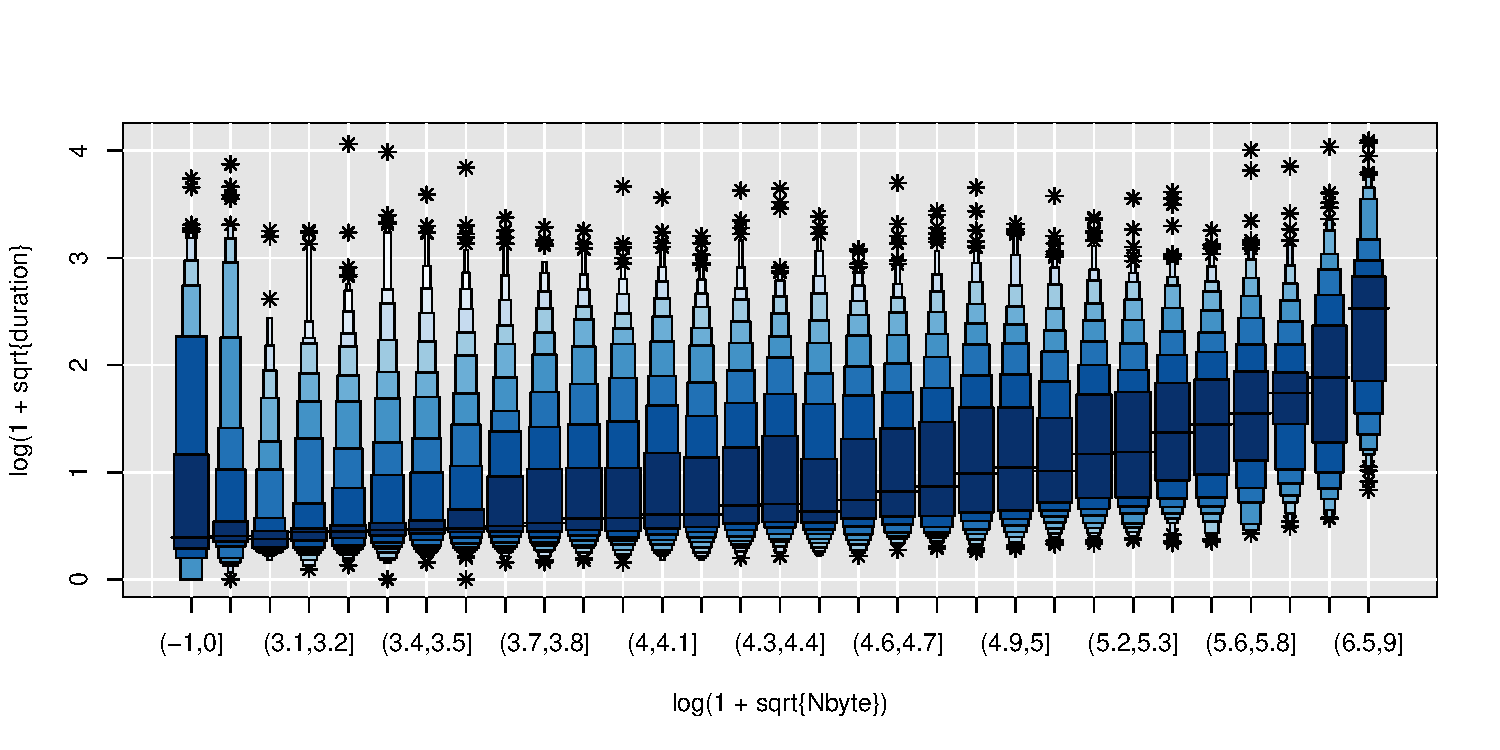
\includegraphics[width=0.75 \linewidth]{lvbox2}

  \caption{Box plots of (log-transformed) duration for
  135,605 Internet sessions, grouped by ranges of (log-transformed) byte
  lengths for the sessions.}
  \label{kkewbox} 
\end{figure}

The conventional box plot is very useful for small or moderate-sized data
sets, but is somewhat inadequate for very large data sets, in two ways. First,
although estimates of quantiles in the tails of a distribution beyond the
quartiles may be imprecise for smaller data sets (and thus probably better not
shown), large data sets afford somewhat more reliable estimates of tail
behavior. Second, because the expected ``some outside rate per sample''
already exceeds 99\% when $n = 700$, the conventional boxplot can be expected
to label increasing numbers of observations as ``outliers''. The letter-value
box plot that we propose addresses both shortcomings for large data sets. In
addition, its construction resembles the original boxplot by displaying only
actual values that occur in the sample. The rules for constructing the letter
value box plot result in the conventional box plot for moderate sized data
sets.

The ``labeled outlier rule'' for conventional boxplots relies 
on the fourths because the rule is then
``unlikely to be adversely affected by extreme
observations'' and ``to minimize the difficulties of masking'' 
(Hoaglin, Iglewicz, Tukey 1986, p.992).
Conventional boxplots rely on the fourths to ensure
insensitivity to the rule governing outlier labeling.
% ``relative insensitivity of summaries and subsequent calculations 
% to unusual observations.'' (citation for this quotation?)  
Hence, the breakdown point of default box plots is 25\%; 
i.e., only if 25\% or more of the data values, all unfavorably
located in one of the tails, are contaminated,
will the summary statistics and outlier identification change.
This high breakdown is one of the valuable features of boxplots.  
Moreover, the relatively low uncertainty in the fourths as 
estimates of the quartiles argues for using the fourths 
in the rule for labeling ``outliers'': the standard deviation 
of the fourths in a Gaussian population equals roughly 
$[(0.25 \cdot 0.75) / (n  \phi(\Phi^{-1}(0.25)))]^{1/2} \sigma$
= $1.362 \sigma / \sqrt{n}$ 
% for a standard Gaussian distribution with
% probability density function $\phi(\cdot)$, 
or a 2-SD uncertainty
of roughly 0.25$\sigma$ for Gaussian samples of size 120 
(David and Nagaraja 2003).
Estimates of the population quantiles beyond the quartiles, when
based on order statistics, are increasingly variable; e.g., for
the same $n = 100$ sample, the 2-SD uncertainty in the eighths
(depth = 13) and sixteenths (depth = 7) is approximately
$ 2 \times 1.607 \sigma / \sqrt{n}$ = $0.32 \sigma$ and
$ 2 \times 1.968 \sigma / \sqrt{n}$ = $0.40 \sigma$, respectively.
Table 1 shows these factors for the standard error formula,
\texttt{SEfactor}, for the first 20 letter values, as well as
the factor in increase in sample size needed for successive
letter values to have the same uncertainty as the fourth.
(For example, the fourths in a sample of size 120 have
a 2-SD uncertainty of 0.25$\sigma$; we would need a sample
of size 1.4$\cdot$120 = 168 for the eighth to have this
same level of uncertainty.)
% by 20--30\% for each subsequent tail area for tail areas 
% 1/8 = 0.125, 1/16 = 0.0625, ..., 1/128 = 0.008, and more beyond
For small samples, then, restricting attention to estimates of only
the population median and quartiles, with some general indication of 
the tail length beyond the quartiles, is likely to be about all the
information that the data can reliably support.



The situation is quite different for large sample sizes. Estimates with
quantiles corresponding to some of the smaller tail areas may be more
reliable, so displays of large data sets can afford to indicate more
confidently estimates of quantiles in the tails. The letter value box plot
incorporates a rule that dictates the number of letter values into the tail
that can be shown with a degree of confidence. In addition, the number of
``labeled outliers'' is based on a function of the last quantile which can be
estimated reliably, which usually limits the number of ``labeled outliers'' to
a reasonable number of observations that can be investigated. ``Outliers'' can
be either (a) genuine, but extreme, observations from the distribution
represented by the bulk of the data; or (b) ``typical'' observations from a
different distribution. The letter-value box plot provides a display of the
data that allows one to better distinguish these two types of observations.

We recall that the theoretical fourths from a sample of \textit{independent}
observations from a single Gaussian population are $\pm 0.6745\sigma$,
yielding an interquartile range, as estimated by the fourth-spread, of
1.3490$\sigma$. Adjacent values (ends of whiskers) therefore lie at $\pm
(0.6745 + 1.5 \cdot 1.3490)\sigma = \pm 2.6980\sigma$, so the box and whiskers
can be expected to cover at least than 99.3\% of the distribution --- leaving
about 0.7\% of the points to be labeled as outliers (and $2.34 \cdot
10^{-04}$\% ``far outliers'') -- hence the approximation in \citet[pg.
34]{dchlv} for the expected number of labeled outliers ($0.4 + 0.007n$). In
the setting of an exponential distribution with unit mean, the theoretical
hinges lie at 0.2877 and 1.3863, so the fourth spread will be roughly 1.0986.
The box and whiskers therefore cover less area, roughly 0.9519, and an
``outlier'' rate of almost 5\% and a ``far-out'' rate of almost 1\%.

The approach of \citet{dchbi}, which labels a fixed number of ``outliers'' (``fixed outside rate'') using a rule that is based on the fourths, avoids this dependence of the expected outside rate on the underlying distribution. Although it avoids the linear dependence of number of ``outliers'' on $n$, it also fails to display any interesting features in the tails. The letter value plot displays such features using data-determined letter values. We review letter value displays in Section~\ref{sec:letter-values} and describe letter value box plots in Section~\ref{sec:lv-boxplots}. Section~\ref{sec:extent} addresses issues of construction (including number of letter values to display). Some proposals for multivariate data and final discussion appears in Sections~\ref{sec:bivariate} and~\ref{sec:summary}.

\section{Letter values}
\label{sec:letter-values}

Let $X_{(1)}$, ... $X_{(n)}$ denote the order statistics from a sample of size
$n$. Per conventional notation, let $\lfloor y \rfloor$ and $\lceil y \rceil$
denote the greatest integer below $y$ and the next integer above $y$,
respectively. The letter values are those order statistics having specific
depths, defined recursively starting with the median. The depth of the median,
$d_1$, of a sample of size $n$ is defined as $d_1 = (1 + n )/2$; the depths of
successive letter values (F = fourths, E = eighths, D = sixteenths, C =
thirty-seconds, ...) are defined recursively as $d_i = (1 + \lfloor d_{i-1}
\rfloor)/2$. (We also will use the letter value itself as the subscript to the
notation for depth; e.g., both $d_1$ and $d_M$ denote the depth of the
median.) The $i^{th}$ lower and upper letter values ($LV_i$) are thus defined
as $L_i = X_{(d_i)}$ and $U_i = X_{(n - d_i + 1)}$. (If the depth is an
integer plus $\frac{1}{2}$, then the lower letter value is defined as the
average of the two adjacent order statistics, $X_{(\lfloor d_i \rfloor)}$ and
$X_{(\lceil d_i \rceil)}$, and similarly for the upper letter value.) The
advantage of this definition for the letter values is that the median of the
sampling distribution for this sample quantile from a continuous distribution
$F(\cdot)$ is very close to $F^{-1} ((i - \frac{1}{3})/(n + \frac{1}{3})$, for
a wide range of $F$, $n$, and $i$ \citep{dchlv}. Because each depth is roughly
half the previous depth, the letter values approximate the quantiles
corresponding to tail areas $2^{-i}$.

The ``labeled outlier rule'' for conventional boxplots relies on the fourths
because the rule is then ``unlikely to be adversely affected by extreme
observations'' and ``to minimize the difficulties of masking'' \citep[pg.
992]{dchbox}. Hence, the breakdown point of default box plots is 25\%; i.e.,
only if 25\% or more of the data values, all unfavorably located in one of the
tails, are contaminated, will the summary statistics and outlier
identification change. This high breakdown is one of the valuable features of
boxplots. Moreover, the relatively low uncertainty in the fourths as estimates
of the quartiles argues for using the fourths in the rule for labeling
``outliers'': the standard deviation of the fourths in a Gaussian population
equals roughly $[(0.25 \cdot 0.75) / (n \phi(\Phi^{-1}(0.25)))]^{1/2} \sigma$
= $1.362 \sigma / \sqrt{n}$ or a 2-SD uncertainty of roughly 0.25$\sigma$ for
Gaussian samples of size 120 \citep{ha.order}. Estimates of the population
quantiles beyond the quartiles, when based on order statistics, are
increasingly variable; e.g., for the same $n = 100$ sample, the 2-SD
uncertainty in the eighths (depth = 13) and sixteenths (depth = 7) is
approximately $ 2 \times 1.607 \sigma / \sqrt{n}$ = $0.32 \sigma$ and $ 2
\times 1.968 \sigma / \sqrt{n}$ = $0.40 \sigma$, respectively.
Table~\ref{tbl:letter-values} shows these factors for the standard error
formula, \texttt{SEfactor}, for the first 20 letter values, as well as the
factor in increase in sample size needed for successive letter values to have
the same uncertainty as the fourth. (For example, the fourths in a sample of
size 120 have a 2-SD uncertainty of 0.25$\sigma$; we would need a sample of
size 1.4$\cdot$120 = 168 for the eighth to have this same level of
uncertainty.) For small samples, then, restricting attention to estimates of
only the population median and quartiles, with some general indication of the
tail length beyond the quartiles, is likely to be about all the information
that the data can reliably support.

\begin{table}[htpb]
  \centering
  \begin{tabular}{llr@{.}lrrr}
  \toprule
  LV & tail area & \multicolumn{2}{l}{rough \%} & $2^j$ & SEfactor & n-equiv*\\ \midrule
   M & .50 & 50&0\% & 2 & 1.253314 \\
   F & .25 & 25& 0\% & 4 & 1.362633 & 1.0\\
   E & .125 & 12& 5\% & 8 & 1.606574 & 1.4\\
   D & .0625 & 6& 25\% & 16 & 1.968236 & 2.1\\
   C & .03125 & 3&13\% & 32 & 2.472133 & 3.3\\
   B & .015625 & 1&56\% & 64 & 3.162020 & 5.4\\
   A & .0078125 & 0&8\% & 128 & 4.101274 & 9.1\\
   Z & .00390625 & 0&4\% & 256 & 5.378300 & 15.6\\
   Y & .001953125 & 0&2\% & 512 & 7.115270 & 27.3\\
   X & .0009765625 & 0&1\% & 1,024 & 9.480641 & 48.4\\
   W & .00048828125 & 0&05\% & 2,048 & 12.706667 & 87.0  \\
   V & .000244140625 & 0&024\% & 4,096 & 17.113727 & 157.7\\
   U & .0001220703125 & 0&012\% & 8,192 & 23.144119 & 288.5\\
   T & .00006103515625 & 0&006\% & 16,384 & 31.408968 & 531.3\\
   S & .000030517578125 & 0&003\% & 32,768 & 42.753381 & 984.4\\
   R & .0000152587890625 & 0&0015\% & 65,536 & 58.346982 & 1833.5\\
   Q & .00000762939453125 & 0&0008\% & 131,072 & 79.808978 & 3430.5\\
   P & .000003814697265625 & 0&0004\% & 252,144 & 109.387241 & 6444.3\\
   O & .0000019073486328125 & 0&0002\% & 504,288 & 150.193933 & 12149.2\\
   N & .00000095367431640625 & 0&0001\% &1,008,576 & 206.552719 & 22977.6\\
  \bottomrule
  \end{tabular}

  \caption{First 20 letter values. Note: \texttt{tail area} is $2 ^{-i}$, $i =
  1, ..., 20$; \texttt{rough}\% rounds $2 ^{-i} \times 100$\% to the first 1
  or 2 nonzero digits; \texttt{odds} expresses tail area as \texttt{1 in}
  $2^i$; ` \texttt{SEfactor} gives the factor for the asymptotic standard
  error of the order statistic (from a Gaussian population, variance
  $\sigma^2$) corresponding to \texttt{tail area}, i.e., $SE(LV) \approx$
  \texttt{SEfactor} $\times \sigma / \sqrt{n}$, where \texttt{SEfactor} =
  $\sqrt{p_i (1-p_i)} / \phi(\Phi^{-1}(p_i))$, $p_i$ = \texttt{tail area} =
  $2^{-i}$. \texttt{n-equiv} = (\texttt{SEfactor}/1.362633)$^2$ which gives
  the factor of increase in sample size for the uncertainty in that letter
  value to be the same as that for the fourth (e.g., need 1.4$n$
  (respectively, 2.1$n$) observations for the eighth (respectively, sixteenth)
  to have the same uncertainty as that of a fourth from a sample of size $n$.
  }
  \label{tbl:letter-values}
\end{table}

% Table~\ref{tbl:counties} illustrates the letter values of the 1980 populations
% and the log populations of the 3068 counties in the continental United States.
% Along with the letter values are shown the midsummaries (average of the upper
% and lower letter values, denoted ``mids'' in Table 2), the midspreads (spread
% between the letter values, denoted ``spread''), and ``pseudo-sigma''
% \citep[pg. 40]{dchlv}, the sample letter-value spread divided by the
% theoretical letter-value spread for a standard Gaussian distribution (e.g.,
% pseudo-sigma based on the fourths is the fourth spread divided by 1.3490). For
% a symmetric population, the midsummaries should be constant, and, for a
% distribution with Gaussian-like tails, the pseudo-sigmas also should be fairly
% stable. Both the midsummaries and the pseudo-sigmas are much more nearly
% constant for the log populations than for the untransformed populations.
% 
% \begin{verbatim}
%                      Table 2
%            Letter value display for 1980
%          populations in 3068 U.S. counties
% 
%     Depth  Lower   Upper      Mid  Spread   pseudo-s
% M  1534.5  218.0   218.0   218.00     0.0     0.0000
% F   767.5  105.0   511.0   308.00   406.0   601.9365
% E   384.0   65.0  1082.0   573.50  1017.0   884.0792
% D   192.5   39.0  2280.0  1159.50  2241.0  1460.7718
% C    96.5   25.0  4572.0  2298.50  4547.0  2441.0384
% B    48.5   17.5  6641.5  3329.50  6624.0  3075.3878
% A    24.5   10.5  9694.5  4852.50  9684.0  4005.6933
% Z    12.5    8.0 14742.5  7375.25 14734.5  5539.1452
% Y     6.5    6.5 18972.5  9489.50 18966.0  6572.5570
% X     3.5    4.5 38316.0 19160.25 38311.5 12369.4452
% W     2.0    4.0 70716.0 35360.00 70712.0 21446.1187
% V     1.5    2.5 72745.5 36374.00 72743.0 20860.5759
% U     1.0    1.0 74775.0 37388.00 74774.0 20383.6663
% 
%              Letter value display for 1980
%          log populations in 3068 U.S. counties
% 
%     Depth  Lower   Upper      Mid  Spread   pseudo-s
% M  1534.5 2.3385  2.3385   2.3385  0.0000     0.0000
% F   767.5 2.0212  2.7084   2.3648  0.6872     1.0189
% E   384.0 1.8129  3.0342   2.4236  1.2213     1.0617
% D   192.5 1.5911  3.3579   2.4745  1.7669     1.1517
% C    96.5 1.3979  3.6601   2.5290  2.2622     1.2144
% B    48.5 1.2429  3.8223   2.5326  2.5794     1.1976
% A    24.5 1.0207  3.9865   2.5036  2.9658     1.2268
% Z    12.5 0.9031  4.1685   2.5358  3.2654     1.2276
% Y     6.5 0.8116  4.2780   2.5448  3.4664     1.2013
% X     3.5 0.6505  4.5512   2.6009  3.9007     1.2594
% W     2.0 0.6021  4.8495   2.7258  4.2475     1.2882
% V     1.5 0.3010  4.8616   2.5813  4.5606     1.3078
% U     1.0 0.0000  4.8738   2.4369  4.8738     1.3286
% \end{verbatim}

Letter values are particularly useful for large data sets, because (a) much of the most valuable information, especially for inference purposes, is contained in the tails (cf.\ Winsor's principle, ``All distributions are normal in the middle''; \citep[pg. 457]{tukey60}); and (b) adjacent letter values have asymptotic correlation $\sqrt{1/2}$ = 0.707 (\citet{mosteller46} cited by \citet[pg. 51--52]{dchlv}. Thus, rather little information concerning tail behavior is lost by considering only the letter values. Figure~\ref{qqpop4} illustrates this retention of tail information in visualizing the distribution of the populations and their logarithms in 3068 continental U.S. counties in 1980 via normal quantile-quantile (QQ) plots (panels A and B, respectively) versus using only the 25 letter values shown in Tables 1 and 2 above (panels C and D, respectively); the bottom panels (letter values only) reveal the advantage of logarithms as well as the top panels (full data set).

\begin{figure}[hbtp]
  \centering
  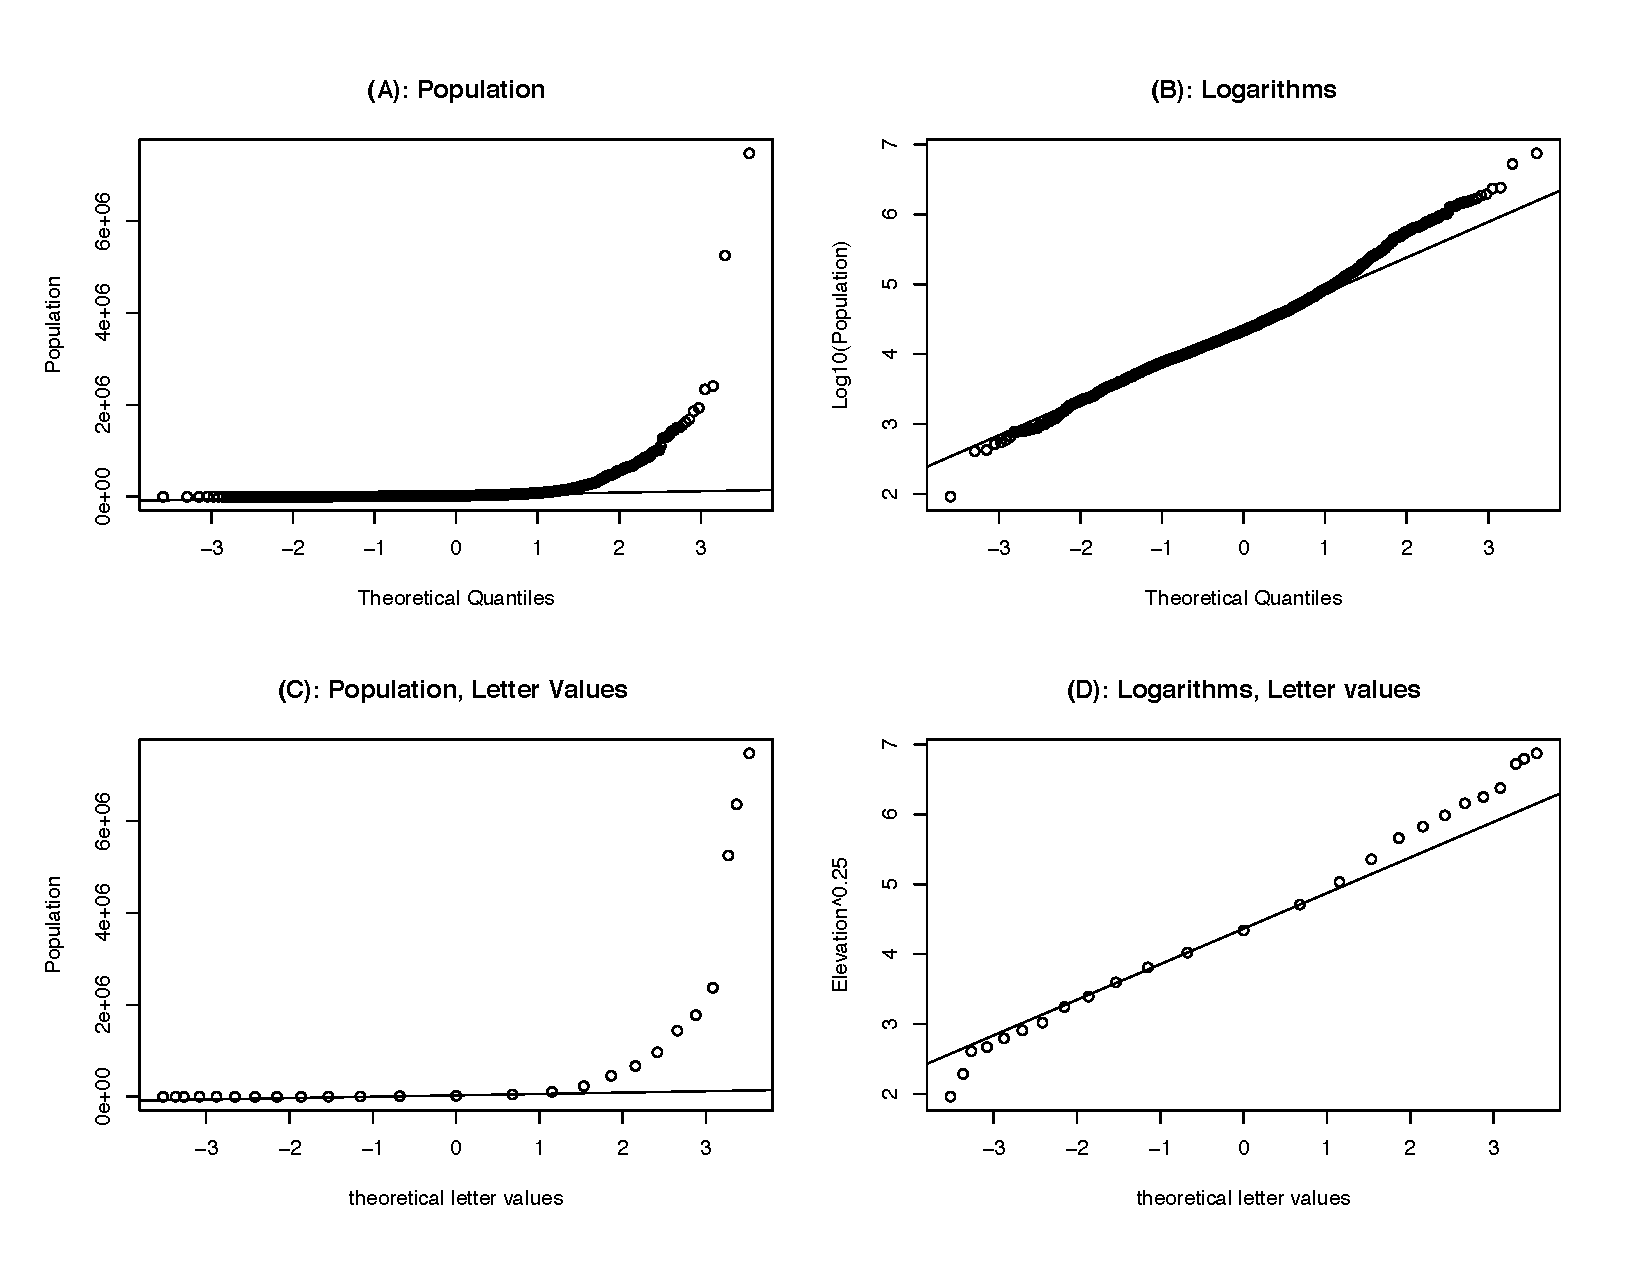
\includegraphics[width = 0.75 \linewidth]{qqpop4}

  \caption{QQ plots on 3068 Continental U.S. county populations (A) and their
  logarithms (B), versus QQ plots (C), (D) using only 25 letter values.}
  \label{qqpop4}
\end{figure}

\section{Letter-value box plots}
\label{sec:lv-boxplots}

Letter-value box plots are based on the letter-value statistics, with one box for each pair of lower and upper letter-values. The median is shown by a vertical line segment, and the innermost box is drawn at the lower and upper fourths, as in the conventional boxplot. An incrementally narrower box is drawn between at the lower and upper eighths, and narrower one still at the lower and upper sixteenths. We continue in this fashion until we reach a box that corresponds to a stopping rule described in the following section; beyond the most extreme box, all observations beyond these limits are identified as individual points. In practice, the software for creating this display proceeds from the outermost box to the innermost (``fourths'') box, so the innermost boxes are shaded more heavily, indicating a higher data density. Boxes with matching heights correspond to the same depths. With this definition, the expected proportion of the sample beyond the end of a box (roughly $1/2^i$) equals the expected proportion between this end and the end of the next bigger box (i.e., roughly $1/2^{i-1} - 1/2^i$ = $(1/2^{i-1})(1 - \frac{1}{2})$ = $1 / 2^i$). When $d_i$ reaches $\log_2 n$, the letter values are the extremes (minimum and maximum).

Letter-value boxplots for three different distributions are shown in Figure~\ref{stackbox}. Each panel displays a sample of 10,000 data points (top = standard Gaussian, middle = exponential with mean 1, bottom = standard uniform), first using the proposed letter-value boxplot up to letter Y, corresponding roughly to tail area $2^{-9}$ = 1/512 (top row), and then with the the conventional boxplot (bottom row). Comparing the left (Gaussian) and right (Uniform) letter value displays, overall \textit{more heavily shaded} displays correspond to distributions with \textit{lighter} tails. This phenomenon is shown more forcefully in Figure~\ref{t-dist} with letter value boxplot for three heavy-tailed distributions: 10,000 samples from a $t$ distribution with 2, 3, 9 degrees of freedom (top rows) and the corresponding boxplots (bottom rows).

\begin{figure}[hbtp]
  \centering
  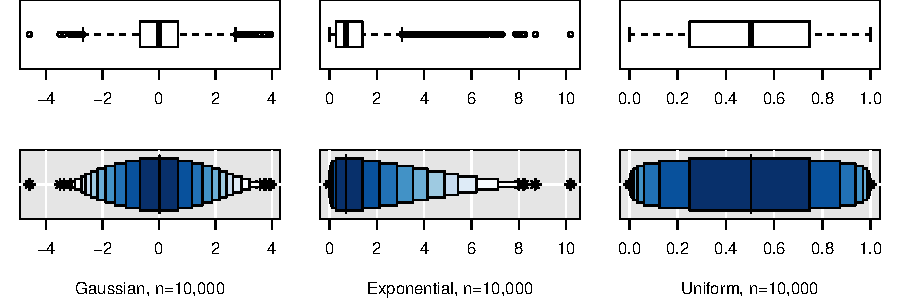
\includegraphics[width = \linewidth]{boxplots}

  \caption{Letter-value box plots (top row) and standard box plots (bottom
  row) for data from three different distributions. Each plot shows 10,000
  data points. From left to right, samples come from $N(0,1)$, $Exp_1$, and
  $U[0,1]$. }
  \label{stackbox}
\end{figure}

\begin{figure}[hbtp]
  \centering
  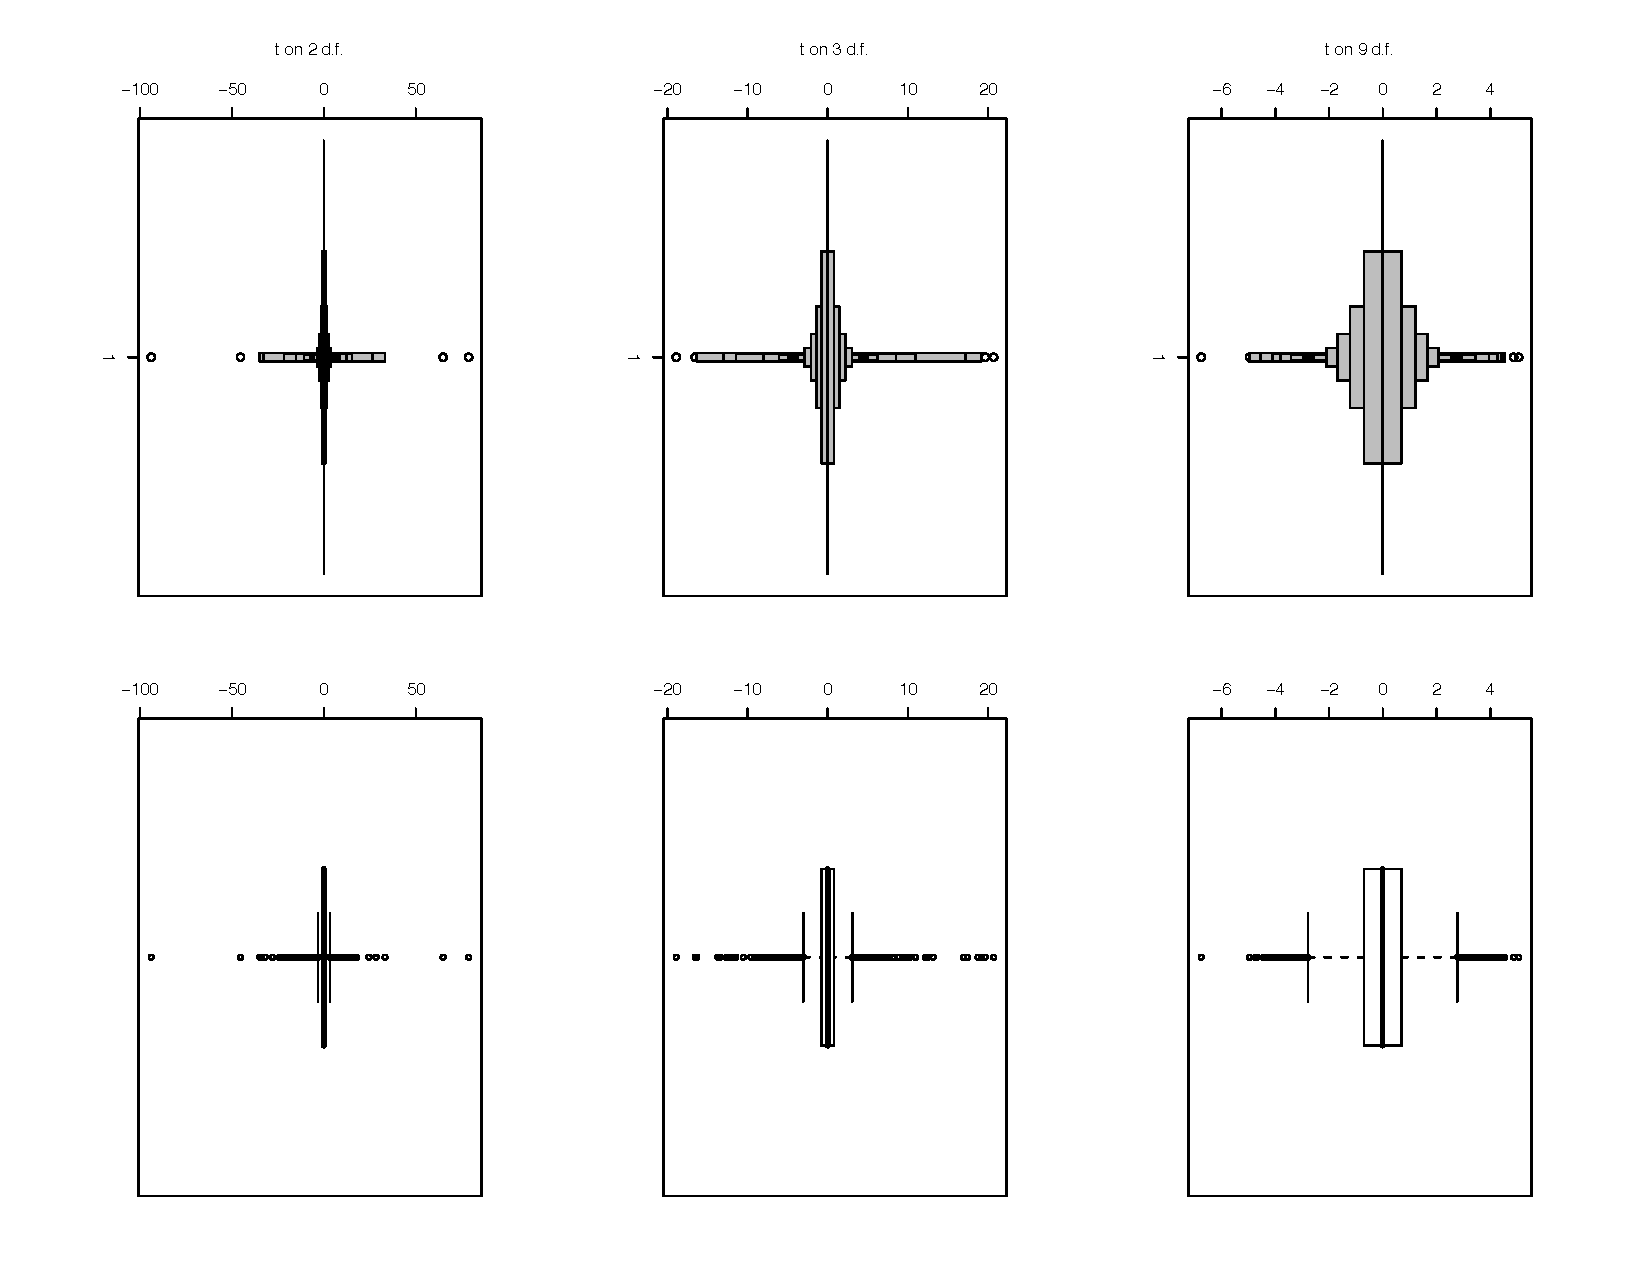
\includegraphics[width = 0.75\linewidth]{tplot2kk}

  \caption{Letter-Value boxplots and standard boxplots for samples of 10,000
  for $t$ distributions on 2, 3, 9 degrees of freedom. Top row: Letter value
  boxplots. Bottom row: Conventional boxplots.}
  \label{t-dist}
\end{figure}

Figure~\ref{lvpops} shows the letter-value boxplots and the conventional boxplots for the 1980 populations and log populations of the 3068 counties in the United States. While the skewness in the distribution of the populations is evident from both the letter-value boxplot and the conventional boxplot, the former shows more clearly that the right tail of the log populations above the median is somewhat more extended than the left tail below the median (i.e., the boxes to the right of the median are slightly longer than those to the left of the median).

\begin{figure}[hbtp]
  \centering
  % \includegraphics[scale=.5]{lvpops}

  \caption{Letter-Value Box Plots and standard box plots for the 1980
  populations and log populations of 3068 counties in the continental United
  States.}
  \label{lvpops} 
\end{figure}

\section{Extent of letter-value boxplots}
\label{sec:extent}

%As indicated in the introduction, a serious drawback to the conventional boxplot for large data sets is the tendency for a very large number of labeled outliers, roughly 0.7\% of the sample size. Figure~\ref{kkewbox} shows a boxplot of a measure of the duration of 135,000 Internet sessions, stratified into 32 groups based on the logarithms of the number of bytes transferred during the session (cf.~\citet{kw06}, for a similar plot). The sample sizes in the 32 boxes range from 1341 (Box\#32) to 7865 (Box\#13), with an average sample size of 4238. With so many observations in each category, the number of labeled outliers is huge --- far too many to investigate individually. This large number makes it difficult to distinguish between genuine ``outliers'' (observations from a different distribution) and merely extreme observations from a distribution with longer tails than the Gaussian.

%\begin{figure}[htbp]
%  \centering
%  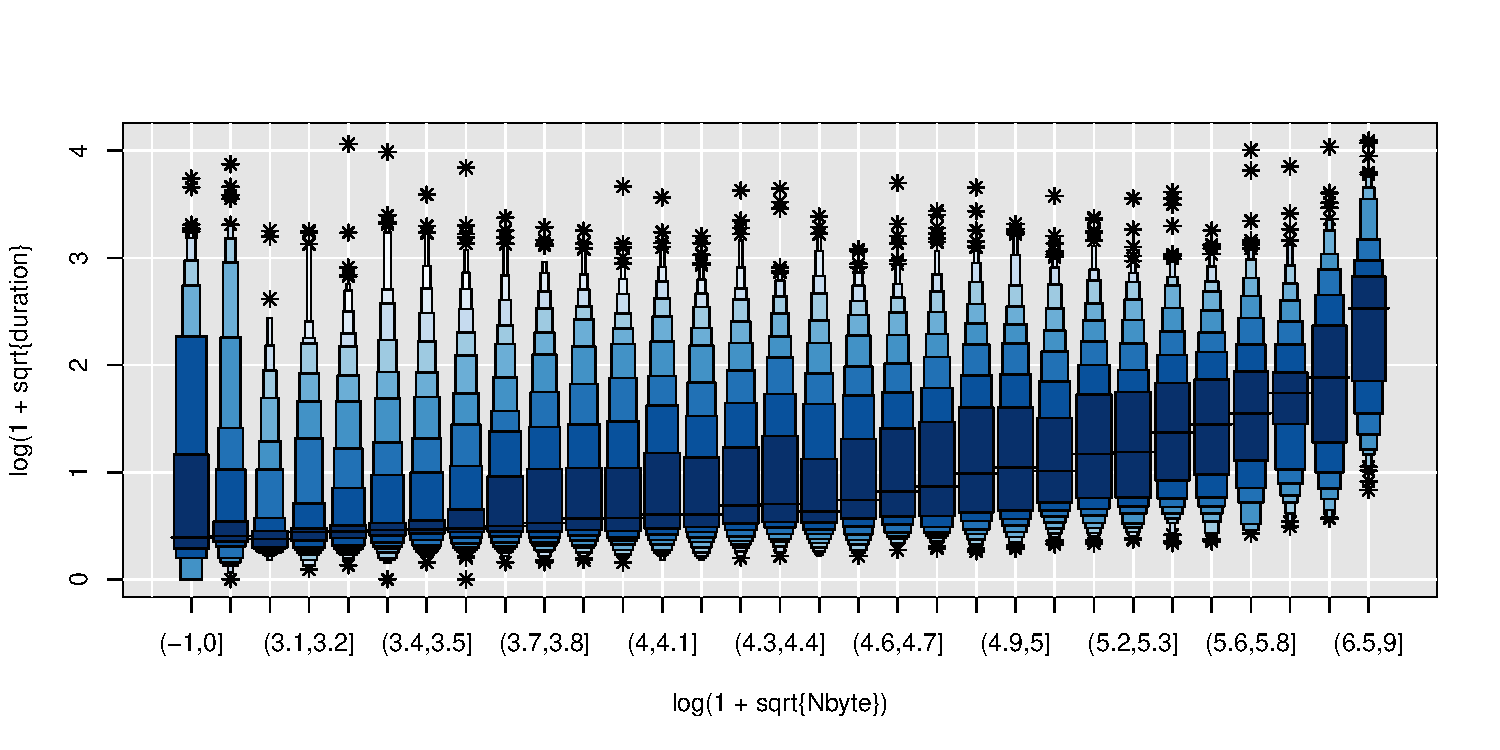
\includegraphics[width = 0.75\linewidth]{lvbox2}

%  \caption{Letter value plots of the boxplots shown in Figure \ref{kkewbox}
%  (transformed durations of 135,000 Internet sessions, grouped by ranges of
%  (transformed) byte lengths).}
%  \label{kkewlv}

%\end{figure}

The standard letter value display stops with that letter value having depth = 1 (i.e., the extremes). In many cases, these extremes could lie far from the rest of the sample, particularly if they are outliers. Just as the whiskers in the conventional boxplot extend only to the adjacent values (observations just inside the inner fences, which can be the extremes in samples with no labeled outliers), the number of boxes in a letter-value boxplot need not extend to the last box corresponding to the extremes. We need a rule to determine the number of boxes to show in a letter-value boxplot, which will determine the number of labeled outliers. In this section, we consider four proposals for such a rule.

In many of the displays in \textit{Exploratory Data Analysis}, Tukey identified 5--8 extreme points. As a rough guideline, we can choose the extent of the letter-value boxplot display so that the last set of boxes encompasses all but the 5--8 most extreme observations. Recall that the depth of the $k^{th}$ letter value, $d_k$, is defined in terms of the previous depth: $d_k = (1 + \lfloor d_{k-1} \rfloor)/2$, which implies that $2 d_{k} -1 \leq d_{k-1} \leq 2 d_k - (1/2)$. If we stop the letter-value boxplot display at $LV_k$ where $k = \lfloor \log_2 n \rfloor - 3$, then we can expect to label 5--8 observations in each tail. For samples of size 10,000 as in Figure~\ref{stackbox}, $k = \lfloor log_2 10000 \rfloor - 4$ = 13 -- 4 = 9, so 9 letter values beyond the median are shown (F, E, D, C, B, A, Z, Y, X -- i.e., down to tail area of roughly 1/1024 $\approx$ 0.001). For the 3068 continental U.S.\ county populations, $k = \lfloor log_2 3068 \rfloor - 4$ = 11 -- 4 = 7, so Figure~\ref{kkewbox} shows 7 letter values (M, F, E, D, C, B, A).

An alternative criterion fixes the number of labeled outliers as a percentage of the overall sample size. Letting $p$ denote this proportion, the last set of boxes to be drawn ends with depths

\begin{equation}
k = \lfloor \log_2 n \rfloor - \lfloor \log_2 (np) \rfloor + 1
\end{equation}

\noindent In effect, conventional box plots use this rule, with $p = 0.007$. This criterion results in the same rule as the previous rule for the samples in Figure~\ref{stackbox} ($n = 10,000$) when $p$ lies between 0.004 and 0.006 (0.4--0.6\%), and in Figure \ref{lvpops} ($n = 3068$) when $p$ lies between 0.011 and 0.020 (1.1--2.0\%).

A third approach is a rule in which the final $k$ is based on the ``trustworthiness'' of the $k^{th}$ letter value as an estimate of the corresponding population quantile. ``Trustworthiness'' can be characterized by the approximate 95\% confidence interval around a given letter value: if the interval overlaps that for the subsequent letter value, then the uncertainty for the given letter value is high enough that we will not display it. Thus, boxes are shown for those letter values whose approximate 95\% confidence intervals exclude the neighboring letter values. Since a letter value can be viewed as the median between the extreme the previous letter value, and since an approximate $1-\alpha$ confidence interval for the median of $m$ values (with $m > 10$) has approximately $0.5 \sqrt{m} z_{1-\alpha/2}$ observations on both sides of the sample median (rounding to the nearest integer), where $z_{1-\alpha/2}$ is the ${1-\alpha/2}$ quantile of a standard Gaussian distribution (\citet[161]{ha.order}, based on the Gaussian approximation to the binomial distribution), this third criterion leads to a particularly straightforward rule.


Consider the upper $k^{th}$ letter value, $LV_k$.  If its
upper 95\% confidence limit does not extend beyond the 
lower 95\% confidence limit for the next letter value, $LV_{k+1}$,
we continue to $LV_{k+2}$; otherwise, the box corresponding to 
$LV_k$ is the last box shown.  
Since approximately $d_{k+1}$ observations lie 
between $LV_k$ and $LV_{k+1}$, 
and the upper 95\% limit for $LV_k$ (respectively, $LV_{k+1}$) has roughly 
$\sqrt{d_{k-1}} \approx \sqrt{2 d_k }$ (respectively, $\sqrt{d_k}$)
observations, this principle requires
$\sqrt{2 d_k} + \sqrt{d_k} < d_{k+1} \approx d_k / 2$, or $d_k > 31.2$.
A rule such as this one with 95\% confidence level often leads to
labeling 5--8 of the most extreme observations on each side,
surprisingly consistent with many of the displays in \textit{EDA}.
[KK: ??? -- it would be more if my calculations are correct. And then the
next sentence would not be right either, nor the subsequent paragraph.
\textbf{Please check}]
Generally, the third rule suggests showing $k$  ``trustworthy'' LVs where
%\begin{eqnarray*}
%0.5 \sqrt{n_k} z_{1-\alpha/2} &<& n_k/4 \\
%\iff \ \ n_k &>&  4 z_{1-\alpha/2}^2 \\
%\end{eqnarray*}
%and since $n_k \approx \frac{1}{2^{k-1}} n$
%%% KK: i think this may need to be fixed.
\begin{equation}
k =  \left \lfloor \log_2 (n) - \log_2 
   \left(4  z_{1-\alpha/2}^2 \right) \right \rfloor + 1
\end{equation}


\noindent This third stopping rule has the obvious advantage that it provides a simple, distribution-free solution. Neither the overall sample size, nor any distribution-related characteristic such as skewness or kurtosis, affects the rule. When $\alpha = 0.05$ (95\% point-wise confidence), the rule leads to showing only those letter values whose depths are at least 10 (i.e., labeling 5--8 observations on each side). Because the first rule is a special case of this third rule, we will consider the use of only stopping rules 2 and 3. Note that $k = 7$ when $n$ is between 492 and 983, which corresponds to letter value A (Gaussian tail area 0.78\%). When $n$ is between 984 and 1966, $k = 8$, corresponding to letter value Z (Gaussian tail area 0.39\%), which is very close to the expected percentage of outliers from a Gaussian sample that are labeled by the conventional boxplot rule (Gaussian tail area 0.35\%).

% KK: I think we need more discussion about the differences 
% between rules 2 and 3, esp since they give diff answers
% depending on $p$.  I also think we'd better number those 2 eqns 
% for later reference.

A fourth rule is a variant of the previous rule, but assesses ``trustworthiness'' in terms of the standard error of the letter value. Table~\ref{tbl:letter-values} shows \texttt{SEfactor}, the factor used for the asymptotic standard error of the letter value for a Gaussian population:

\begin{equation}
SE(LV_i) \approx \sigma \sqrt{p_i \cdot (1 - p_i)/ n} / \phi(\Phi^{-1}(p_i)) 
 = (SEfactor) \sigma / \sqrt{n} \, ,
 \, \, \, p_i = 2^{-i} \, .
\label{SELV}
\end{equation}

\noindent When $i = 2$ ($p_i = 0.25$, fourths) and $n = 120$, this standard error is approximately 0.125$\sigma$; when $n = 186$, it is 0.10$\sigma$, and when $n = 743$, it is 0.05$\sigma$. Thus, a rough 2-SE interval around the fourth is roughly 0.25$\sigma$, 0.2$\sigma$, or 0.1$\sigma$, respectively, as $n$ increases from 120 to 186 to 743. How many more letter values can be shown with the same level of uncertainty when $n$ increases? For illustration, consider only the last (and most stringent) criterion, where 2$SE$ $\approx$ 0.1$\sigma$. If $n \geq 1032$, the asymptotic 2-SE uncertainty in $LV_3$, the eighth (E), using the formula in (\ref{SELV}), does not exceed 0.1$\sigma$. For the same precision in $LV_4$ (sixteenth), one needs $n \geq 1550$.

Table~\ref{tbl:lv-error} lists the letter values and the ranges on $n$ for which the uncertainty displayed up to a given letter value does not exceed 0.5$\sigma$, 0.25$\sigma$, 0.20$\sigma$, and 0.10$\sigma$. For example, when $n$ = 10,000 and a 2-SD uncertainty around the letter value no greater than 0.20$\sigma$, one can show up to letter value 10 (X, 1/1024), but only up to letter value 7 (A, 1/128) for uncertainty of that does not exceed 0.10$\sigma$. Figure~\ref{figyy} plots the columns in Table~\ref{tbl:lv-error} on a $\log_10$ scale, which shows that the logarithm of the sample size is approximately linear in the letter value number. This rule is very similar to rule (1) when the desired uncertainty in the letter values does not exceed 0.25$\sigma$.

The different rules provide the user with choices depending on the desired precision in the letter values shown. The current implementation of the letter-value box plot display uses rule 3 as a default option.

\begin{table}
  \begin{center}
  \begin{tabular}{lrrrrr}
    \toprule
      &  i &    0.5 &     .25 &     0.2 &      0.1 \\
    \midrule
    M &  1 &     25 &     101 &     157 &      628 \\
    F &  2 &     30 &     119 &     186 &      743 \\
    E &  3 &     41 &     165 &     258 &     1032 \\
    D &  4 &     62 &     248 &     387 &     1550 \\
    C &  5 &     98 &     391 &     611 &     2445 \\
    B &  6 &    160 &     640 &    1000 &     3999 \\
    A &  7 &    269 &    1077 &    1682 &     6728 \\
    Z &  8 &    463 &    1851 &    2893 &    11570 \\
    Y &  9 &    810 &    3240 &    5063 &    20251 \\
    X & 10 &   1438 &    5752 &    8988 &    35953 \\
    W & 11 &   2583 &   10333 &   16146 &    64584 \\
    V & 12 &   4686 &   18744 &   29288 &   117152 \\
    U & 13 &   8570 &   34282 &   53565 &   214260 \\
    T & 14 &  15784 &   63137 &   98652 &   394609 \\
    S & 15 &  29246 &  116983 &  182785 &   731141 \\
    R & 16 &  54470 &  217880 &  340437 &  1361748 \\
    Q & 17 & 101914 &  407654 &  636960 &  2547840 \\
    P & 18 & 191449 &  765796 & 1196557 &  4786227 \\
    O & 19 & 360931 & 1443726 & 2255822 &  9023287 \\
    N & 20 & 682624 & 2730498 & 4266403 & 17065610 \\
    \bottomrule
    
  \end{tabular}
  \end{center}
  \caption{caption}
  \label{tbl:lv-error}
\end{table}


\begin{figure}[hbtp]
  \centering
  % \includegraphics[scale=.6,angle=270]{figyy}

  \caption{Plot of $\log_10 n$ versus letter value number to ensure a 2-SD
  uncertainty in displayed letter values of no more than 0.50 (5, black), 0.25
  (3, red), 0.20 (green, 2), 0.10 (blue, 1). Fitted lines have slopes 0.25 and
  intercepts 0.754, 1.356, 1.550, and 2.152, respectively. Data from Table 4.}
  \label{figyy} 
\end{figure}

\section{Bivariate letter value plots}
\label{sec:bivariate}

\citet{bagplots} proposed the ``bagplot'' as a two-dimensional version of the boxplot, using location depths (introduced by \citet{tukey75}) to define analogues of the median and fourths, and then connecting the points corresponding to the fourth-depths via linear segments. 
Example here [Heike]
The location depth $ldepth(p,Z)$ is defined for an arbitrary point $p \in \Reals^2$, relative to a set of $n$ points $Z$ = \{$z_i = (x_i, y_i)$, $i = 1,...,n$\}, as the smallest number of $z_i$'s contained in any closed halfplane with boundary line through $p$. That is, if one were to pass a line in the plane through $p$ and keep track of the smaller of the two numbers of $z_i$ on either side of the line as the line is rotated through every angle to its opposite side ($180^o$), then the location depth of that point $p$ relative to $Z$ is the smallest of all the numbers. The analog of the one-dimension median in two dimensions using location depth would thus be that point $p_M$ for which $ldepth(p_M, Z)$ is largest (e.g., $n/2$). If such a $p$ is not unique, then the ``depth median'' is defined as the ``center of gravity'' of all points $p$ for which $ldepth(p,Z)$ is largest. Recall that a property of the fourths for a univariate sample is that the interval between the lower and upper fourth contains one-half of the data. Thus, an analog of the box for the bagplot was defined as the set of points for which $ldepth(p,Z) = \lfloor n/2 \rfloor$ (more precisely,...) Algorithms for conveniently fast computation of bivariate letter values for a bivariate letter value box plot is currently under development.

\section{Summary}
\label{sec:summary}

The advantages of the letter value box plot are:

\begin{itemize}
\item they are based on actual data values 
\item they are simple to compute from the letter value display
\item they convey further information about tail behavior beyond the whiskers
\item for large data sets, fewer observations are labeled as ``outliers'' 
compared to a conventional boxplot (roughly 0.7\%)
\item their construction does not depend on a smoothing parameter.
\end{itemize} 

% \appendix
% \section{Implementation}
% 
% The Appendix contains the R code for implementing these letter-value boxplots. The code has been posted also on \texttt{http://statlib.cmu.edu}. Further information about the code and its implementation are available from the first author.
% 
% \begin{verbatim}
% LVboxplot <- function(x, k = NULL, perc = NULL, alpha = 0.95, horizontal = T,
%   col = T, ...) 
% \end{verbatim}
% 
% \begin{itemize}
% \item[x] vector of data values to be displayed
% \item[k] number of letter-value statistics shown.
% \item[perc] percentage of data points to be shown individually (as outliers) outside the letter-value boxes.  {\tt perc} is used only if {\tt k} is not specified.
% \item[alpha] significance level, if neither {\tt k} nor {\tt perc} is specified.  {\tt alpha} is used in Rule 3 for the number of boxes to show.  If used, confidence intervals around each letter value  excludes neighboring letter value at significance level {\tt alpha}.
% \end{itemize}
% 
% \noindent The function returns a list with three components:
% 
% \begin{itemize}
% \item[letter.val] matrix of values (lower and upper) of all {\tt k}
%   letter values, including depth of each.
% \item[conf.int] $2k-1 \times 2$ matrix of confidence intervals for 
%   all letter values using significance level as specified in {\tt alpha}.
% \item[outliers] list all identified points (outliers in standard box plot).
% \end{itemize}

\bibliographystyle{asa}
\bibliography{references}
\end{document} 
